\chapter{Dettagli implementativi e di deploy}\label{chap:impl}
In questo capitolo sono descritti alcuni dettagli relativi all'implementazione dell'interprete che è stato realizzato in Alchemist. In particolare verrà descritta la gerarchia delle classi definite all'interno dell'incarnazione e successivamente le proprietà e le funzionalità di quelle principali: Incarnation (AgentIncarnation), Node (AgentsContainerNode), Action (AbstractAgent).

Successivamente sono descritti gli strumenti utilizzati per supportare lo sviluppo di questo progetto: Gradle per la gestione delle librerie all'interno di Alchemist, GitHub per la gestione del repository e del codice sorgente, Travis CI per il monitoraggio di eventuali anomalie prodotte.

Infine, è presente una panoramica relativa alla costruzione della configurazione di una simulazione in Alchemist. Vengono descritte le varie parole chiave che possono essere utilizzate per caratterizzare la simulazione e, al termine, viene fornito un esempio di una configurazione per la simulazione.

\section{Note implementative}
Dopo aver già descritto i tratti principali dell'interprete per il modello ad agenti implementato all'interno di Alchemist, in questa sezione sono mostrate alcune caratterizzazioni più specifiche di come è stata realizzata l'incarnazione, con un focus verso le principali entità del modello e sulla struttura delle classi .
Inoltre verrà fatta una descrizione degli strumenti di sviluppo utilizzati per l'elaborazione del progetto.

\subsection{Gerarchia delle classi}
Precedentemente in questo lavoro si è accennato alle classi dell'incarnazione utilizzate per realizzarla limitandosi però solamente ad alcune informazioni generiche. In questa sezione l'obiettivo è quello di descrivere in maniera più accurata le classi, il funzionamento e le loro gerarchie all'interno dell'implementazione dell'interprete che è stata realizzata.

L'immagine presente in Figura \ref{fig:UMLGerarchiaClassi} mostra lo schema UML delle classi realizzate.
%crea l'ambiente figura;
\begin{figure}[ht] % [h] sta per here, cioè la figura va qui
%\begin{center} % centra nel mezzo della pagina la figura
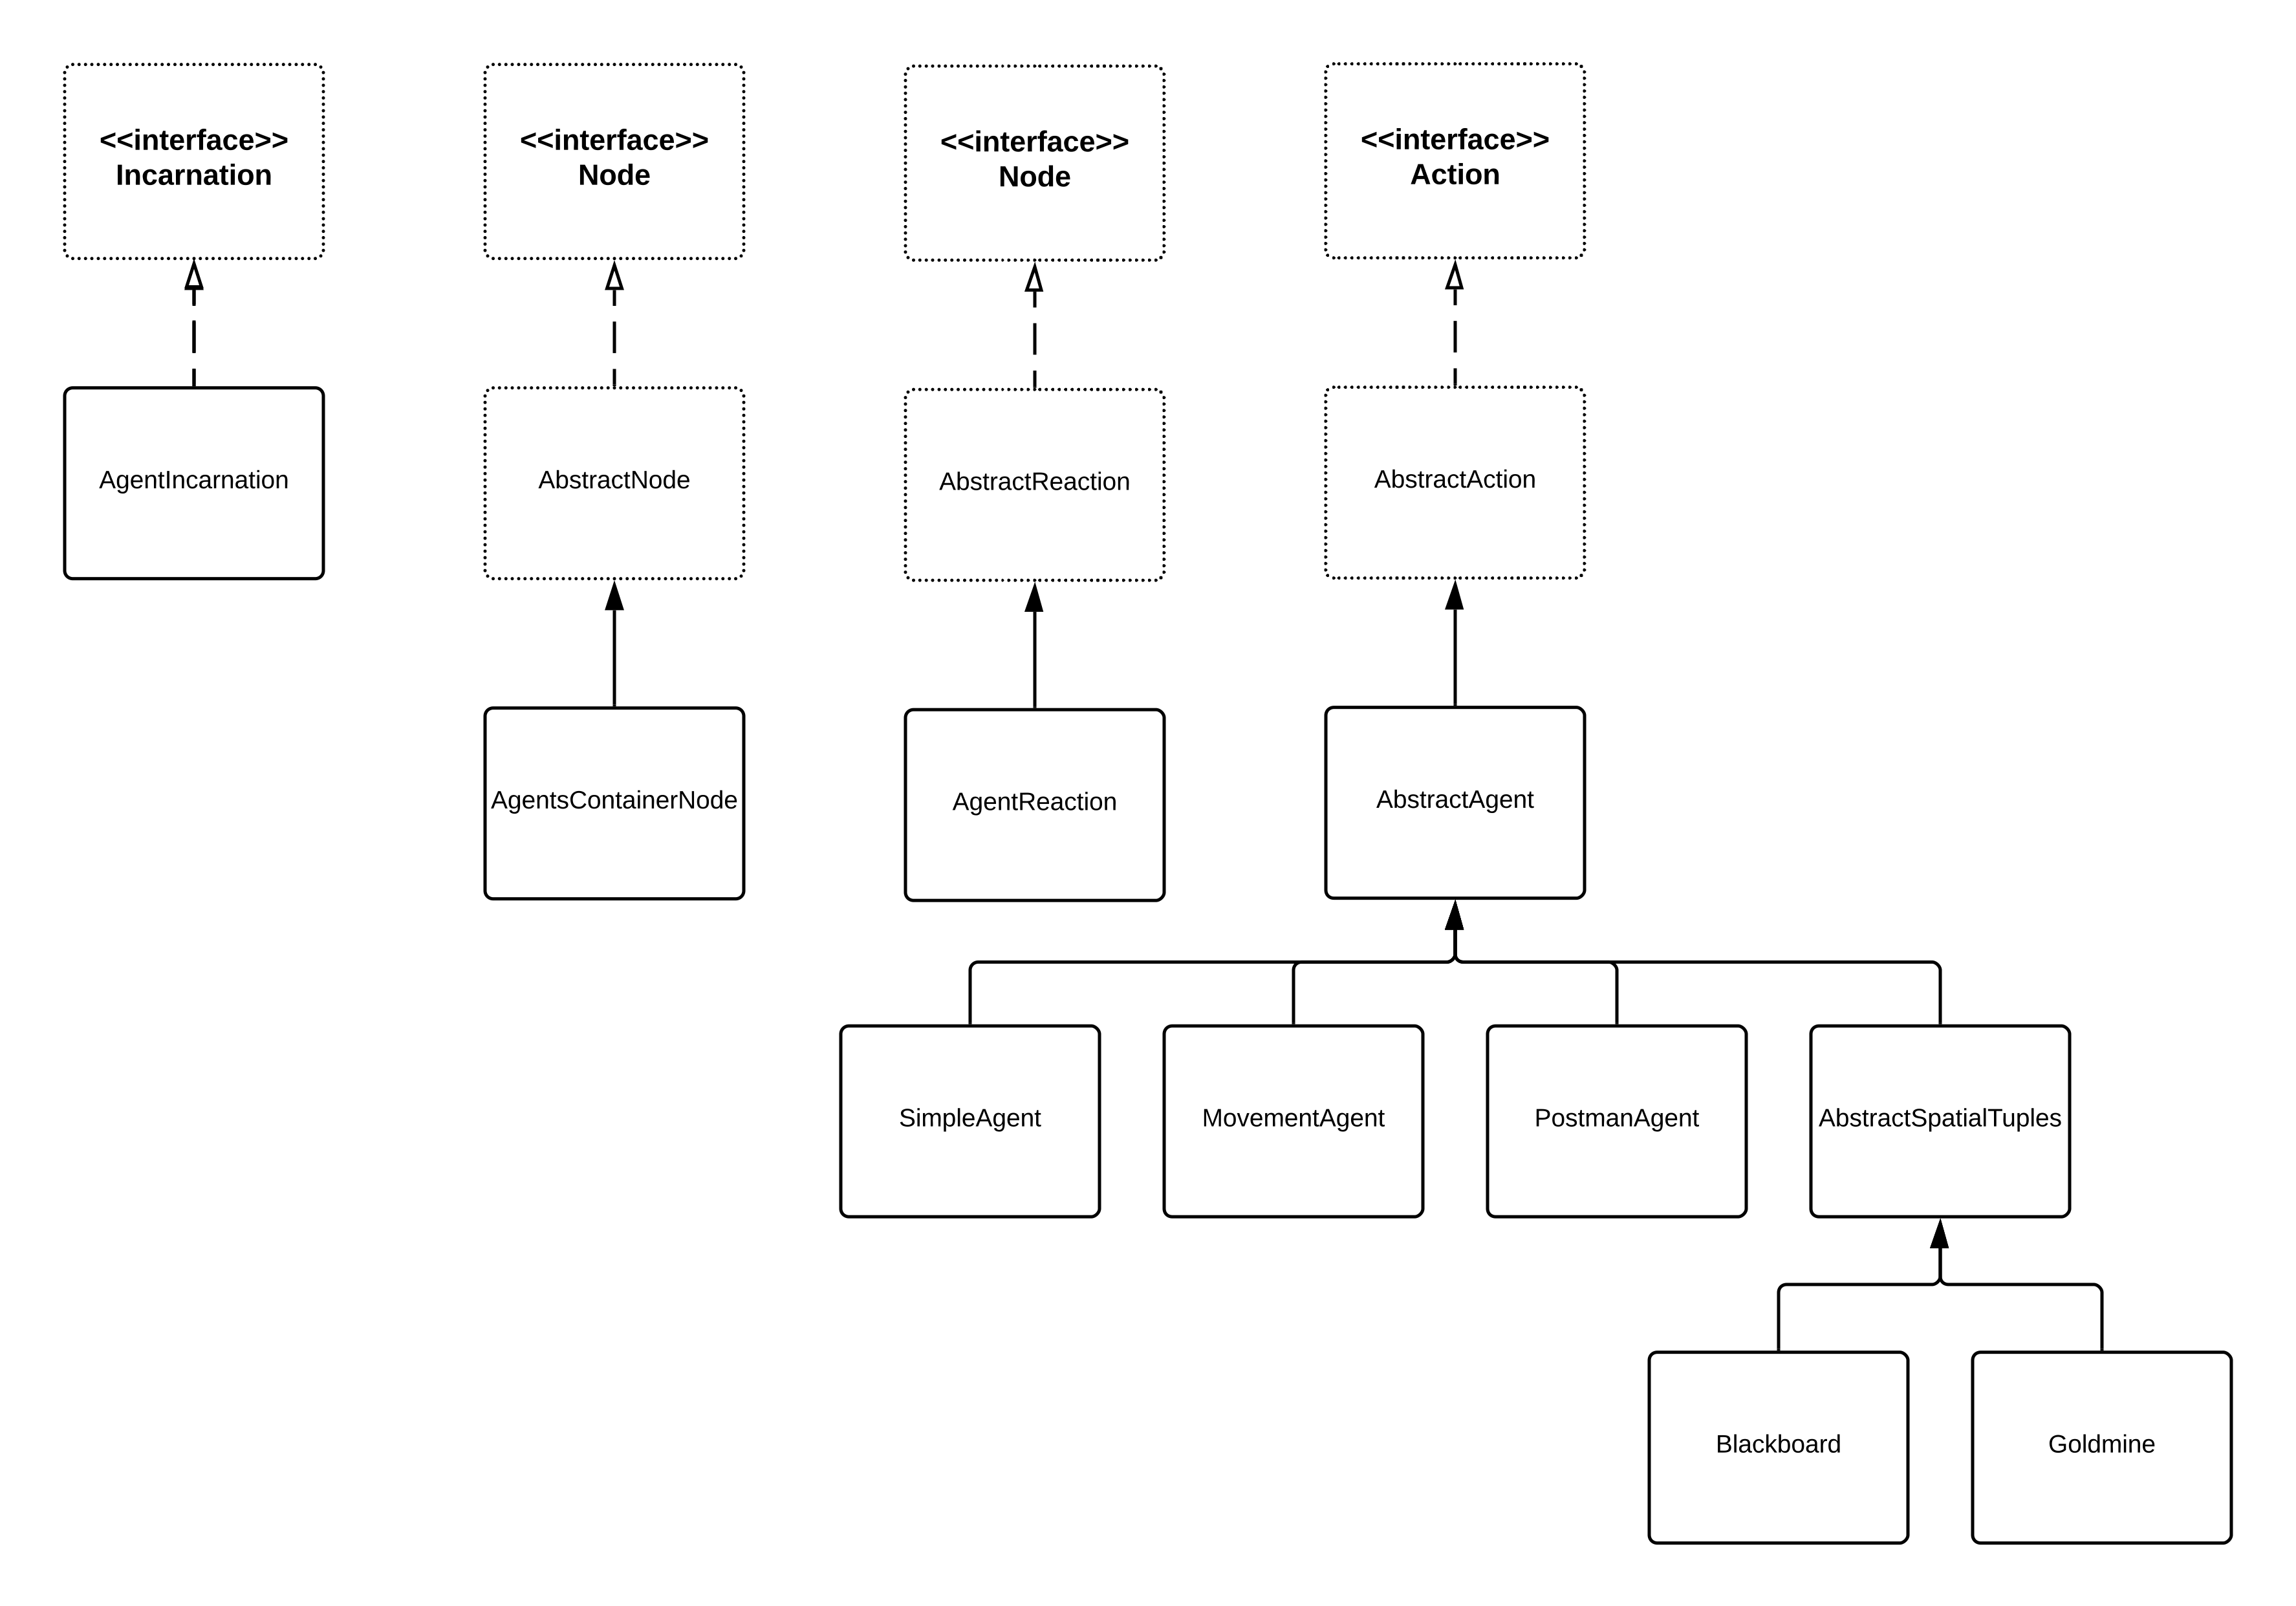
\includegraphics[width=15cm]{images/UML_agenti.png} % inserisce una figura larga 12.5cm
% inserisce la legenda ed etichetta la figura con \label{fig:prima}
\caption[Ricostruzione UML della gerarchia delle classi]{Ricostruzione UML della gerarchie delle classi} \label{fig:UMLGerarchiaClassi}
%\end{center}
\end{figure}

Lo schema rappresenta in modo informale la gerarchia di alcune classi e mostra la loro struttura ereditaria; quest'ultima comprende alcune classi o interfacce già implementate in Alchemist e pronte per essere utilizzate. I riquadri con il bordo tratteggiato distinguono le classi che non sono state definite per questa specifica incarnazione ma sono già presenti all'interno del simulatore: questo rende possibile utilizzare e lavorare con il simulatore in maniera più efficiente. Le restanti classi, rappresentate in riquadri con un bordo continuo, sono le classi implementate per realizzare, in questa specifica incarnazione di Alchemist, l'interprete per il nuovo linguaggio ad agenti.
\\
Per quanto riguarda le frecce, quelle con la linea tratteggiata stanno ad indicare la relazione `implements', ovvero che una certa classe implementa l'interfaccia indicata, mentre quelle con il tratto continuo significano `extends', ovvero che una classe estende le proprietà e le funzionalità di quella da cui deriva.

Nello schema si può notare che la classe dell'incarnazione è stata realizzata partendo direttamente dall'implementazione dell'interfaccia: la struttura di questa classe verrà descritta nella sezione \ref{sctn:AgentIncarnation}.
\\
Diversamente, per il Nodo e la Reazione si è scelto di estendere le rispettive classi astratte già presenti all'interno di Alchemist, le quali al loro interno implementano l'interfaccia di riferimento. La classe del nodo verrà spiegata più in dettaglio nella sezione \ref{sctn:AgentsContainerNode}, mentre per la reazione, che è l'entità individuata per rappresentare l'agente, è stata implementata la classe senza conferire particolare caratteristica poichè il core dell'agente è realizzato, come già accennato nella sezione \ref{sctn:InvocazioneEsecuzioneIntenzioni}, in un'entità contenuta al suo interno, ovvero l'Azione.
\\
Come si può vedere dallo schema l'azione è l'entità che ha avuto il maggior numero di implementazioni. Per la realizzazione dell'Azione si è partiti descrivendo le funzionalità generiche dell'agente all'interno di una classe astratta per fornire un'esemplificazione e una base di partenza da poter utilizzare con poco sforzo o eventualmente ampliare per realizzare comportamenti specifici.
Ad esempio, per l'integrazione del modello SpatialTuples è stata estesa la classe base dell'agente per realizzare una nuova classe astratta (AbstractSpatialTuple) che, allo stesso modo della classe padre, offre la possibilità di utilizzare degli spazi di tuple avendo già una solida base di partenza. La classe dell'agente è descritta nella sezione \ref{sctn:AbstractAgent}.
Le altre classi implementate a partire dalla classe AbstractAgent sono implementazioni specifiche di agenti che sono state utilizzate per la realizzazione di simulazioni di scenari di test. Le classi che estendono AbstractSpatialTuple sono anch'esse realizzate come agenti ma incarnano il comportamento degli spazi di tuple.

\subsection{L'incarnazione}\label{sctn:AgentIncarnation}
Per realizzare la classe principale dell'incarnazione, e solo per questo caso, è stata implementata direttamente la corrispondente interfaccia, ovvero Incarnation.
Questa interfaccia definisce i metodi per poter implementare in maniera specifica ogni singola entità del meta-modello di Alchemist. All'interno della classe AgentIncarnation, che implementa appunto l'interfaccia Incarnation, sono state implementate le varie funzioni che, in fase di esecuzione, saranno opportunamente richiamate dal simulatore. Qui di seguito viene fornita una breve descrizione di come sono stati implementati i metodi definiti nell'interfaccia.

All'interno del metodo per la creazione di un oggetto dell'entità Molecola viene creata un'istanza della classe SimpleMolecule, implementazione già presente all'interno di Alchemist, che a partire da una stringa (utilizzata come identificativo) crea una corrispondente molecola.

Per quanto riguarda la Distribuzione Temporale, come accennato nella sezione \ref{sctn:SpostamentoNodo}, viene utilizzata la classe DiraComb, già implementata in Alchemist, che permette di creare eventi periodici ad una distanza temporale definita tramite un parametro.

Per creare il Nodo sono utilizzati i riferimenti all'Environment, che è utilizzato per gestire funzionalità come lo spostamento e il vicinato, e al RandomGenerator, il quale è impiegato per ottenere randomicità negli agenti. All'interno del metodo per la creazione di un Nodo è invocato il costruttore della classe AgentsContainerNode che ne fornisce un'istanza: l'oggetto creato è poi restituito all'applicazione per essere utilizzato durante la simulazione.

Per poterne gestire lo spostamento, come accennato nella sezione \ref{sctn:SpostamentoNodo}, all'interno di ogni nodo è stato inserito uno specifico agente incaricato di questo compito. L'operazione di inserimento avviene all'interno del metodo per la creazione del Nodo; dopo aver ottenuto un'istanza di AgentsContainerNode si crea una Reazione, che al suo interno conterrà l'azione per gestire il movimento, la quale è aggiunta al nodo prima di essere restituito.
\\
Per creare questa Reazione, viene eseguito lo stesso procedimento descritto all'interno dell'apposito metodo definito all'interno della classe ma variando le funzioni invocate e la tipologia di alcuni oggetti istanziati.

Per creare una `normale' Reazione viene per prima cosa creata un'istanza della classe AgentReaction e poi invocati i metodi per creare le istanze di azioni e condizioni, passando gli opportuni parametri che specificano, tra gli altri, la classe dell'oggetto da istanziare. A questo punto, gli oggetti ottenuti dall'invocazione delle due funzioni, vengono inseriti all'interno dei rispettivi set della reazione, la quale viene infine ritornata.
\\
Nel caso della reazione per lo spostamento, sono create sul momento le istanze degli oggetti che andranno a crearla e con il seguente ordine:
\begin{itemize}
\item[1.] TimeDistribution, tramite invocazione del metodo $createTimeDistribution$ implementato nella classe AgentIncarnation;
\item[2.] AgentReaction;
\item[3.] MovementAgent;
\item[4.] Condition, tramite invocazione del metodo $createCondition$ implementato nella classe AgentIncarnation.
\end{itemize}
%L'ordine è importante poichè la distribuzione è utilizzata all'interno della reazione, che a sua volta è utilizzata per creare l'azione e la condizione ad essa relativi.
Con la stessa modalità descritta appena sopra, le istanze di azione e condizione sono inserite all'interno di specifici set della reazione che, infine, viene inserita nel nodo. Questa è una reazione particolare poichè viene costruita `manualmente' (non tramite apposita funzione) e viene inserita `nativamente' nel nodo per comandare il suo movimento.
\\
Inoltre, un passaggio che viene eseguito nella funzione di creazione della Reazione, è l'invocazione di un metodo, implementato nel nodo, il quale registra ogni nuovo agente all'interno di una struttura dati. Questo passaggio consente ad ogni nodo di mantenere traccia di tutti gli agenti presenti al suo interno e rende possibile recuperare il riferimento di ogni agente, anche esternamente rispetto al nodo a cui appartiene, in qualsiasi momento.
L'agente per lo spostamento non viene inserito nella struttura dati descritta e potrà essere individuato solamente recuperandolo dal nodo tramite le funzioni messe a disposizione da Alchemist.

La creazione della condizione è gestita in modo che questa risulti sempre vera e che quindi, secondo il meta-modello di Alchemist, vengano sempre scatenate le azioni collegate alla relazione a cui appartiene quella certa condizione. L'oggetto condizione che viene restituito dal metodo $createCondition$, invocato dall'interprete, è un'istanza della classe AbstractCondition che viene completata implementando la definizione del contesto (che impatta sulle performance della simulazione) e della condizione di validità (che come accennato poc'anzi è impostata per essere sempre vera).

Infine parliamo della creazione di oggetti dell'entità Azione. Per la creazione di queste istanze in base ad una valutazione del parametro ricevuto, che è stato passato dalla creazione della reazione, viene definita quale sia la classe dell'istanza da creare.
L'istanza dell'oggetto opportunamente inizializzata viene quindi ritornata per essere utilizzata all'interno di una reazione.
Al momento sono gestiti i casi per le seguenti classi:
\begin{itemize}
\item SimpleAgent
\item PostmanAgent
\item BlackboardAgent
\item GoldmineAgent
\end{itemize}


\subsection{Il contenitore degli agenti - Nodo}\label{sctn:AgentsContainerNode}
Il nodo, nell'implementazione dell'interprete realizzata, è uno spazio (o contenitore di agenti) che gestisce i comportamenti dell'agente verso l'esterno, come ad esempio lo spostamento del nodo stesso e l'esecuzione di azioni esterne, ma implementa anche una serie di funzioni utili alla gestione della comunicazione tra agenti (recupero dell'elenco degli agenti nel vicinato, gestione dei messaggi fra agenti). Il nodo, come detto precedentemente, è definito tramite la classe AgentsContainerNode creata estendendo la classe astratta AbstractNode che a sua volta implementa l'interfaccia Node.

All'interno della classe sono definite le proprietà che contengono l'ambiente, il generatore random, i valori per gestire lo spostamento del nodo ed una struttura per il monitoraggio degli agenti presenti al suo interno.
Le istanze di Environment e RandomGenerator sono create all'interno del core di Alchemist e poi passate al costruttore della classe che le memorizza all'interno della classe. %, dopo averle registrate, inizializza inoltre la variabile che mantiene il tempo per dell'ultimo aggiornamento della posizione.
La struttura dati scelta è una mappa formata da una serie di coppie di valori composti da una chiave, che rappresenta il nome dell'agente, ed il valore, che è il riferimento stesso dell'agente. Attraverso questa struttura il nodo è in grado di recuperare il riferimento di ogni singolo agente presente al suo interno; questa implementazione, come vedremo di seguito, è stata molto utile per produrre nuove funzionalità specifiche implementate nel nodo.

Oltre alle proprietà, all'interno della classe sono presenti i metodi per la gestione della posizione, della mappa che monitora gli agenti e del vicinato calcolato in base a diversi criteri.

\`E quindi possibile impostare o recuperare i valori di direzione e velocità oppure ottenere la posizione stessa del nodo. Ovviamente è presente il metodo mostrato nel Codice sorgente \ref{lst:ImplementazioneAggiornamentoPosizioneNodo} che effettua il calcolo per ottenere le coordinate della nuova posizione del nodo.
Inoltre, è implementato il metodo $updateAgentsPosition()$ che innesca l'aggiornamento dei fatti, quali posizione e distanza dagli altri agenti, per ogni agente all'interno del nodo. Secondo l'implementazione attuale, questo metodo viene invocato solamente dall'agente `Movement', inserito alla creazione del nodo, che, nel suo ciclo di ragionamento, ha come unico compito quello di invocare questo metodo per scatenare l'aggiornamento. Gli agenti quindi verranno aggiornati quando lo scheduler di Alchemist farà eseguire il ciclo di ragionamento dell'agente `Movement'.

Per la gestione della mappa, utilizzata per il monitoraggio degli agenti, sono presenti due metodi: uno per effettuare l'inserimento, invocato come descritto nella sezione \ref{sctn:AgentIncarnation} durante la creazione di istanze dell'entità Reazione, e uno per ottenere la struttura completa.

Il concetto di vicinato viene gestito da Alchemist attraverso la funzione di linking-rule, che utilizza il parametro `network-model' se opportunamente impostato in fase di configurazione della simulazione.
Lato implementativo, è sufficiente richiedere all'Environment di fornire tutti i nodi presenti nel vicinato con i quali è poi possibile effettuare altre operazioni come, ad esempio, ottenere la distanza tra i vari nodi e recuperare gli agenti presenti in ogni nodo, utilizzando l'apposita mappa.
\\
Lo stesso meccanismo è utilizzato per recuperare e operare negli spazi di tuple, definiti utilizzando l'estensione SpatialTuples. In questo caso, non è stato sufficiente il solo recupero di tutti i nodi ma sono stati applicati i filtri per ottenere solo gli agenti la cui istanza derivi da AbstractSpatialTuple.
Secondo la scelta implementativa effettuata, è necessario specificare due insiemi differenti per le diverse primitive invocabili sullo spazio di tuple: la scrittura è fatta su un solo spazio di tuple, ovvero quello più vicino, mentre la lettura su tutti quelli del vicinato.
Il secondo caso è il più immediato poichè si recupera l'elenco di tutti gli agenti presenti nei nodi del vicinato e si verifica solamente che l'istanza dell'agente sia un'implementazione della classe astratta AbstractSpatialTuple. Ogni agente che corrisponde a questa condizione viene aggiunto ad una lista, la quale è poi ritornata come output.
\\
Diversamente, per quanto riguarda la scrittura, serve individuare lo spazio di tuple più vicino, recuperandolo tramite la mappa di agenti del nodo che lo contiene. Utilizzando l'ambiente, vengono confrontate le distanze di tutti i nodi rispetto a quello attuale e, si recupera quello più vicino che contiene almeno un'agente che sia istanza della classe astratta AbstractSpatialTuple. Di quel nodo viene selezionato il primo agente trovato che corrisponde ai canoni poichè verosimilmente, in base alle scelte implementative, in ogni nodo vi è un solo spazio di tuple.

Un altro metodo implementato all'interno della classe AgentsContainerNode è $postman()$ per la gestione dei messaggi, in modo simile a quanto realizzato per lo spostamento del nodo. Un'agente dedicato, chiamato `Postman' invoca un metodo che recupera tutti i messaggi in uscita da tutti gli agenti dell'ambiente e li consegna al corretto destinatario. Maggiori dettagli di questa funzionalità sono descritti nella sezione \ref{sctn:DettaglioImplementazioni}.

Inoltre, sempre all'interno della classe del nodo, è stato scelto di implementare il metodo, invocabile dalla teoria dell'agente, per la gestione delle azioni esterne.
La scelta di implementare questa funzionalità all'interno del nodo è dovuta alla sua posizione nell'ambiente rispetto al modello e al mapping scelto poichè è lo snodo in cui si ha la possibilità di interagire sia con l'ambiente che con gli agenti di altri nodi. Si è quindi implementato il metodo $executeExternalAction(String action)$ all'interno del quale, in base all'azione ricevuta come parametro, viene selezionata una serie di operazioni che portano al raggiungimento di quella certa azione. Come invocare funzionalità implementate in Alchemist dalla teoria è mostrato nella sezione \ref{sctn:DettaglioImplementazioni}.

\subsection{L'agente - Azione}\label{sctn:AbstractAgent}
L'agente è il punto centrale dell'incarnazione che è stata realizzata, dal quale sono partiti tutti i ragionamenti per il design dell'interprete e la mappatura del modello ad agenti sul meta-modello di Alchemist.

Come già detto precedentemente, l'agente è stato associato alla Reazione che però non è essa stessa l'entità operativa, ovvero quella che viene eseguita periodicamente, ma solo il contenitore. L'entità Azione è la parte che il simulatore richiama attivamente per l'esecuzione se le condizioni, anch'esse contenute nella Reazione, validano le proprie clausole.

Per la realizzazione della classe dell'agente si è scelto, anche in questo caso, di partire da un'implementazione già fornita da Alchemist, ovvero dalla classe astratta AbstractAction.
\\
La scelta successiva è stata quella relativa al design della classe da implementare. Dopo un'accurata analisi è stato scelto di realizzare, invece che un'implementazione definitiva, una classe astratta che descrive le proprietà base dell'agente e ne implementa le funzionalità principali (inizializzazione dell'agente e gestione di messaggi, di `belief base', di intenzioni e di operazioni negli spazi di tuple), lasciando comunque al programmatore la scelta della caratterizzazione dell'agente. La scelta di creare una classe astratta è dovuto al fatto di non voler dare nessuna implementazione del ciclo di ragionamento ma fornire implementazioni dei comportamenti e azioni basilari che lo compongono: in questo modo è possibile facilmente definire nuovi comportamenti o creare agenti partendo da quelli già realizzati.
\\
Non sono quindi implementati i metodi $execute()$, $cloneAction(node, reaction)$, definiti dall'interfaccia Action, dalla cui implementazione è caratterizzato il comportamento dell'agente. In particolare, il metodo $execute()$, che è quello che rappresenta il ciclo di ragionamento, è invocato periodicamente dal core di Alchemist (questo perchè le Condizioni collegate alla stessa Reazione sono impostate per essere sempre vere) per lo svolgimento delle azioni.

All'interno della classe sono definite le seguenti proprietà: due code per i messaggi (una per quelli in entrata e una per quelli in uscita), il motore tuProlog, lo stack contenente gli identificativi delle intenzioni presenti nella teoria, riferimenti alla reazione e al generatore random.

La classe astratta dell'agente gestisce, inoltre, la teoria dell'agente e sfrutta il motore tuProlog importato tramite l'apposita libreria `alice.tuprolog'. Attraverso questo componente è possibile caricare una teoria ed effettuare interrogazioni della stessa permettendo all'agente di operare raccogliendo i risultati per creare intenzioni o inserire nuove informazioni.

Per inizializzare un agente sono state definite una serie di operazioni posizionate poi all'interno dei metodi $initializeAgent()$ e $initReasoing()$.
Questi due metodi hanno come obiettivo quello di inizializzare l'agente: il primo lo fa dalla parte dell'interprete mentre il secondo configura l'inizializzazione dello stato iniziale dell'agente.
Entrambi, per la corretta configurazione dell'agente in relazione all'implementazione attuale, dovrebbero essere richiamati all'interno del ciclo di ragionamento solamente una volta, ovvero alla prima iterazione, per completare la configurazione dell'agente iniziata nel costruttore.

All'interno del metodo $initializeAgent()$ viene caricata nel motore tuProlog la libreria dell'agente, quella descritta nel capitolo precedente e che implementa il linguaggio definito in questo lavoro di tesi, a cui segue il caricamento della teoria specifica che definisce il comportamento di un certo agente. Successivamente, sempre all'interno dello stesso metodo, viene eseguita la registrazione di oggetti Java all'interno della teoria (questa azione verrà descritta in dettaglio nella sezione \ref{sctn:DettaglioImplementazioni}) e l'inserimento all'interno della teoria dell'agente del fatto $self(nome\_agente)$ che completa la procedura di inizializzazione da parte dell'interprete.
\\
Nel metodo $initReasoning()$ viene eseguita una sola operazione, ovvero l'invocazione della regola $init$ che permette al programmatore dell'agente di eseguire una configurazione dello stato iniziale dell'agente.
Al termine di queste due operazioni si può considerare l'agente completamente inizializzato e pronto per reagire a tutti i possibili eventi per cui è stato programmato.

All'interno dell'agente, utilizzando il generatore random, è definita una proprietà per la gestione della casualità che è un'istanza della classe LevyDistribution, definita nel package `org.apache.commons.math3.distribution', la quale permette di creare una distribuzione random a partire da un randomizzatore. Questa distribuzione è messa a disposizione insieme al randomizzatore per fornire all'agente casualità da utilizzare nelle sue operazioni. Ad esempio può essere utilizzata per generare valori per la velocità e la direzione del nodo che contiene l'agente.

Per quanto riguarda lo scambio di messaggi, l'agente implementa i metodi per inserire e recuperare i messaggi dalle sue code che sono richiamati opportunamente dall'agente `Postman' descritto nella sezione \ref{sctn:DettaglioImplementazioni}.
Internamente l'agente definisce una classe per i messaggi con all'interno le proprietà per memorizzare mittente, destinatario e contenuto.
Le operazioni che vengono effettuate sui messaggi dall'agente sono due: una per leggerli, recuperando un messaggio dalla coda in entrata, ed una per inviarli, posizionando il messaggio nella coda di uscita.
Per la lettura è stata implementata una funzione che recupera un messaggio, se presente, nella coda di quelli in entrata e sfruttando il contesto recupera la corretta regola, definita nella teoria dell'agente, da cui ottenere la lista di operazioni per creare un'intenzione. Quanto appena detto viene fatto seguendo la modalità descritta nella sezione \ref{sctn:InvocazioneEsecuzioneIntenzioni} e che sarà poi mostrata più nel dettaglio nella sezione \ref{sctn:DettaglioImplementazioni}.

La funzione implementata per la gestione della `belief base' utilizza i fatti generati dall'invocazione delle regole definite nella sezione \ref{sctn:ImplementazioneLinguaggio} e recuperandoli tramite opportune interrogazioni della teoria dell'agente. Allo stesso modo della lettura del messaggio, utilizzando il contesto del fatto, ovvero il contenuto del belief recuperato, viene ottenuta la regola, definita nella teoria dell'agente, dalla quale sono recuperate le operazioni da inserire nella lista dell'intenzione da creare.

Nel capitolo precedente è stata descritta la procedura che porta all'esecuzione e alla rimozione delle intenzioni presenti nella teoria dell'agente. Però non è stato descritto qual è il procedimento che porta alla creazione di un'intenzione.
Nella sezione \ref{sctn:DettaglioImplementazioni} verrà mostrato come è possibile creare un'intenzione partendo da un termine e poi cercando nella teoria dell'agente una regola adatta ad esso.

Il funzionamento delle azioni interne è stato descritto in maniera approfondita nella sezione \ref{sctn:GestioneAzioni} utilizzando come esempio l'azione per l'invio di un messaggio. All'interno della classe dell'agente è quindi presente questa funzione $executeInternalAction(action)$ con la quale l'interprete implementato esegue una sequenza di operazioni che portano al compimento dell'azione. Come invocare funzionalità implementate in Alchemist dalla teoria è mostrato nella sezione \ref{sctn:DettaglioImplementazioni}.

L'aggiornamento della posizione che avviene nell'agente è scatenato dal metodo $updateAgentsPosition()$ del nodo che a sua volta viene innescato dall'esecuzione dell'agente `Movement'. All'interno dell'agente sono definite le due funzionalità che sono richiamate dal metodo del nodo: $updateAgentPosition(position)$ e $updateAgentsDistances()$. La prima si occupa dell'aggiornamento nella `belief base' dei fatti relativi alle nuove coordinate e della creazione di un'intenzione relativa all'evento di aggiornamento della posizione per consentire all'agente di reagire al nuovo stato.
La seconda funzione adegua le distanze dell'agente corrente rispetto agli altri agenti del vicinato inserendo due diversi fatti: se l'agente è un nuovo vicino viene inserito il belief con il nome e la distanza tra i due agenti; altrimenti se l'agente era già presente all'interno del vicinato il belief inserito contiene anche la vecchia distanza tra i due agenti, fornendo quindi un'informazione utile in alcuni domini applicativi.

Come già accennato nella sezione \ref{sctn:ImplementazioneSpatialTuples}, all'interno dell'interprete è stato implementato anche il modello Spatial Tuples.
All'interno dell'agente sono state implementate due funzioni per l'invio e la ricezione di richieste per gestire la comunicazione con lo spazio di tuple.
\\
Per quanto riguarda il metodo per l'invio della richiesta, l'agente recupera i fatti presenti all'interno della teoria e per ognuno costruisce una richiesta formata da un termine, l'istanza dell'agente e la primitiva($in$, $rd$, $out$) che esegue quel termine. Come già descritto, la scelta implementativa è stata quella di inserire la richiesta di scrittura sullo spazio di tuple più vicino, mentre quelle delle altre primitive su tutti gli spazi di tuple del vicinato.
\\
Il metodo che consente all'agente di ricevere il risultato della richiesta è stato implementato fornendo in ingresso solamente un parametro, il termine recuperato dallo spazio di tuple. In questo modo all'interno della teoria dell'agente sarà sufficiente trovare una regola $onResponseMessage(T)$, dove $T$ è il parametro ricevuto, idonea al contesto per poi creare una nuova intenzione da inserire tra quelle da eseguire.

\subsection{Dettaglio implementazioni}\label{sctn:DettaglioImplementazioni}
In questa sezione verranno descritti alcuni dettagli relativi all'implementazione realizzata quali il funzionamento dell'agnete `Postman', la referenziazione e l'utilizzo di oggetti Java in tuProlog, la creazione delle intenzioni.

\subsubsection{Agente `Postman'}
Per la gestione dei messaggi, l'agente implementa al suo interno i metodi per prelevarli e inserirli da entrambe le code. Internamente utilizza solo le funzioni per leggere nuovi messaggi e per aggiungere quelli da inviare nella coda di quelli in uscita.
Il vero e proprio scambio di messaggi è demandato all'agente `Postman' creato specificatamente per questo compito. Questo agente nel suo ciclo di ragionamento ha come unico compito quello di invocare la funzione $postman()$ implementata nel nodo, e mostrato nel Codice sorgente \ref{lst:ImplementazioneFunzionePostman}.
\lstset{
  numberstyle=\footnotesize\color{black},
  basicstyle=\ttfamily,
  breakatwhitespace=true,
  breaklines=true,
  captionpos=b,
  keepspaces=true,
  numbers=left,
  numbersep=7pt,
  showspaces=false,
  showstringspaces=false,
  showtabs=false,
  tabsize=2,
  frame=tb,
  language=Java,
  commentstyle=\color{gray},
  keywordstyle=\color{blue},
  stringstyle=\color{red}
}
\medskip
\begin{lstlisting}[firstnumber=1,label={lst:ImplementazioneFunzionePostman},caption={Implementazione funzione Postman}]
Map<String, AbstractAgent> agents =
	new LinkedHashMap<>();
List<AbstractAgent.OutMessage> outMessages =
	new ArrayList<>();

// Get all agents from each node in the environment
this.environment.getNodes().forEach(node -> {
    agents.putAll(
    		((AgentsContainerNode) node).getAgentsMap()
    	);
});

// For each agent takes outgoing messages
agents.forEach((agentName, agent) -> {
    outMessages.addAll(agent.getOutMsgs());
});

// Send each message to the receiver
outMessages.forEach(message -> {
    agents.get(message.getReceiver()).addInMsg(message);
});
\end{lstlisting}

Quando opportunamente invocato, questo metodo recupera tutti i nodi dell'ambiente (quindi non solamente quelli del vicinato) e da ognuno ne estrae, utilizzando l'apposita struttura, gli agenti, i quali vengono uniti insieme per creare un'unica lista. Quest'ultima viene iterata per recuperare tutti i messaggi in uscita presenti in ogni agente e poi per ogni messaggio viene estrapolato il nome del destinatario. Attraverso il nome si risale al riferimento dell'agente sul quale viene invocato il metodo per inserire il messaggio nella coda di quelli in entrata.
\\
L'esecuzione del metodo è previsto che venga fatta una sola volta e globalmente: per questo è stata implementata la classe PostmanAgent, implementazione della classe AbstractAgent, la quale effettua nel suo ciclo di ragionamento solamente questa operazione.

\subsubsection{Referenziazione e utilizzo oggetti Java in tuProlog}
Per poter referenziare oggetti Java all'interno della teoria dell'agente è stata sfruttata una funzionalità di tuProlog attraverso l'utilizzo della libreria Object-Oriented.
L'esclusivo approccio di tuProlog mantiene i due modelli computazionali chiaramente separati, in modo che né lo stile dichiarativo di Prolog né lo stile imperativo/OO di Java si influenzino a vicenda \cite{2p-alpnews2013}.
Questa funzione è fornita dalla libreria JavaLibrary, la quale è organizzata su due punti:
\begin{itemize}
   \item una mappatura tra tipi di oggetto e tipi Prolog adeguati \cite{2p-alpnews2013};
   \item un set di predicati per eseguire operazioni su oggetti Java \cite{2p-alpnews2013}.
\end{itemize}

Nel Codice sorgente \ref{lst:BindingOggettiJavaIntuProlog} è mostrato come sono state configurate le due variabili $agent$ e $node$ disponibili nella teoria tuProlog e che si riferiscono alle istanze di agente e nodo presenti nel simulatore Alchemist.
\begin{lstlisting}[firstnumber=1,label={lst:BindingOggettiJavaIntuProlog},caption={Binding oggetti Java in tuProlog}]
// tuProlog engine
Prolog engine = new Prolog();
// tuProlog OOLibrary
Library lib = engine.getLibrary("alice.tuprolog.lib.OOLibrary");
...
// Object reference for internal actions
((OOLibrary) lib).register(
	new Struct("agent"), this
);

// Object reference for external actions
((OOLibrary) lib).register(
	new Struct("node"), this.getNode()
);
\end{lstlisting}
Nella classe astratta dell'agente è stata recuperata la libreria ad oggetti utilizzando l'istanza del motore tuProlog.
\`E stata poi utilizzata la funzione $register(id, obj)$ messa a disposizione dalla libreria che permette di registrare al suo interno identificativi di variabili utilizzabili in tuProlog riferiti ad oggetti Java.
Come si può vedere nel Codice sorgente \ref{lst:BindingOggettiJavaIntuProlog} recuperato dalla classe dell'agente, all'interno della libreria viene prima registrata la variabile $agent$ referenziata alla classe stessa e poi la variabile $node$ riferita al nodo, recuperato attraverso il riferimento dell'agente.
\\
Lato tuProlog l'utilizzo di questo strumento è molto intuitivo. Dopo aver registrato gli oggetti, nel modo appena mostrato, è sufficiente invocare i metodi implementati all'interno della classe come mostrato nel Codice sorgente \ref{lst:UtilizzoBindingIntuProlog}. Qui di seguito daremo una descrizione degli esempi mostrati.
Nella prima riga viene fatta un'invocazione di una funzione $doSomething()$ che non ha parametri in ingresso.
Nel secondo esempio l'invocazione riguarda la funzione $doSomethingWithParams(string, term)$ che riceve parametri di tipo String e Term. La signature del metodo Java è fondamentale: se il tipo degli oggetti attesi non corrisponde a quelli passati il metodo risulterà non invocato.
Nell'ultimo caso è mostrato come si possono invocare funzioni che ritornano un risultato come output e come quest'ultimo possa essere inserito all'interno di una nuova variabile da poter utilizzare all'interno della regola.

\lstset{
  basicstyle=\ttfamily,
  captionpos=b,
  numbers=none,
  frame=tb,
  stringstyle=\color{black}
}
\medskip
\begin{lstlisting}[firstnumber=1,label={lst:UtilizzoBindingIntuProlog},caption={Utilizzo riferimenti oggetti Java in tuProlog}]
% no params
agent <- doSomething

% with params
agent <- doSomethingWithParams(`term',V)

% using return result
agent <- getNextRand returns R,
TMP is R * 0.5.
\end{lstlisting}

\subsubsection{Creazione intenzioni}
Le intenzioni sono utilizzate per la gestione dei comportamenti dell'agente. Un'intenzione, come detto nella sezione \ref{sctn:AgentiBDI}, rappresenta un'insieme di azioni che l'agente deve compiere per completare un certo comportamento, e cioè per reagire ad eventi per cui l'agente è stato programmato.

Le azioni all'interno dell'interprete vengono create quindi in relazione agli eventi o alla creazioni di nuovi goal.
La procedura per creare un'intenzione inizia dalla definizione della struttura del template utilizzata per cercare il piano adatto per reagire a quell'evento. Invocando la funzione $createPlanStruct(term)$, dove $tem$ è l'evento per il quale si sta creando l'intenzione, viene restituito un oggetto strutturato come mostrato nel Codice sorgente \ref{lst:OggettoStrutturaPiano}.
\lstset{
  numberstyle=\footnotesize\color{black},
  basicstyle=\ttfamily,
  breakatwhitespace=true,
  breaklines=true,
  captionpos=b,
  keepspaces=true,
  numbers=left,
  numbersep=7pt,
  showspaces=false,
  showstringspaces=false,
  showtabs=false,
  tabsize=2,
  frame=tb,
  language=Java,
  commentstyle=\color{gray},
  keywordstyle=\color{blue},
  stringstyle=\color{red}
}
\medskip
\begin{lstlisting}[firstnumber=1,label={lst:OggettoStrutturaPiano},caption={Oggetto che definisce la struttura del piano}]
return new Struct('<-', term, new Var('GUARD'), new Var('BODY'))
\end{lstlisting}

L'oggetto $struct$ che è stato creato viene poi passato all'invocazione del metodo $createIntention(term, errMsg)$, dove $errMsg$ è una stringa contenente un messaggio utilizzato in caso di errore.
All'interno del metodo viene utilizzata la struttura all'interno del motore tuProlog per interrogare la teoria dell'agente e recuperare una lista di piani rilevanti (nella teoria sono definiti come fatti). \\
\\
Successivamente per ogni piano recuperato viene controllata la veridicità della guardia attraverso l'utilizzo di regole opportunamente definite nella libreria tuProlog dell'agente che è stata creata. La guardia definisce il contesto e quindi determina se un piano rilevante è anche applicabile.
Se la guardia non è verificata il piano viene scartato altrimenti si passa al recupero del corpo, ovvero la lista di azioni che deve essere eseguita.
\\
Le azioni possono essere descritte in due diverse modalità: si può trovare una lista di azioni, caso in cui viene recuperato un fatto che descrive un piano per reagire ad un evento, oppure può essere il corpo di una regola. Nel primo caso la lista viene semplicemente recuperata mentre nel secondo caso il corpo viene trasformato in una lista di azioni.
\\
Ottenuta la lista di azioni $body$ si inizia la vera e propria creazione dell'azione: per prima cosa viene generato un identificativo univoco $id$ e successivamente viene creata la struttura $intention(id,body)$ che poi è inserita all'interno della teoria dell'agente. Se l'inserimento è completato con successo l'$id$ è inserito anche nella lista lato Java che mantiene gli identificativi di tutte le intenzioni presenti nella teoria dell'agente, e che è utilizzata per gestire l'esecuzione delle intenzioni con metodo Round-Robin.


\subsection{Tool di sviluppo}
Per lo sviluppo di questo progetto, oltre all'utilizzo di ambienti applicativi per l'implementazione dell'interprete, ci si è appoggiati ad altri strumenti esterni per la gestione e verifica del codice sorgente prodotto. Qui di seguito sono citati e descritti gli strumenti utilizzati.

\subsubsection{Gradle}
Gradle è un sistema open source che permette l'automazione dello sviluppo focalizzandosi su flessibilità ed efficienza \cite{Gradle}. I vantaggi offerti sono:
\begin{itemize}
\item alta personalizzazione: è modellato in modo da poter essere personalizzabile ed esteso;
\item veloce: completa task velocemente riutilizzando gli output da precedenti esecuzioni, processando solamente i cambiamenti ed eseguendo task in parallelo;
\item potente: è lo strumento ufficiale per la build di Android e fornisce supporto per i più popolari linguaggi e tecnologie.
\end{itemize}
All'interno di Alchemist, questo tool di sviluppo è stato utilizzato per la gestione dell'intero progetto e non solo per librerie esterne. Essendo presenti all'interno del progetto principale varie incarnazioni o sotto-progetti per parti in comune è necessario gestirne le dipendenze in modo efficace. Attraverso un'opportuna configurazione, sia del file principale che di quelli presenti in ogni progetto interno, sono stati gestiti una serie di meccanismi per l'importazione al fine di realizzare le incarnazioni.

\subsubsection{GitHub}
GitHub è un servizio di hosting per progetti software. Le principali funzionalità che offre sono:
\begin{itemize}
\item hosting del codice
\item revisione del codice
\item gestione dei progetti
\item integrazioni
\item documentazione
\end{itemize}

Alla base vi è sicuramente la possibilità di ospitare codice sorgente all'interno di vari repository che possono essere pubblici, privati o open source con la possibilità di versionare ogni singola modifica e tenendo traccia di chi l'abbia prodotta \cite{GitHub}.
Tramite questo meccanismo è più semplice revisionare il codice e gestire eventuali risoluzioni di bug o miglioramenti, potenzialmente suggeriti anche da persone esterne se il repository lo permette.
\\
GitHub permette di mantenere una documentazione allegata al progetto consentendo di creare singole pagine collegabili tra loro oppure caricare l'intera documentazione posizionata nella cartella `docs/' nel branch `master' \cite{GitHub}.
\\
Un'altra funzionalità è quella della gestione del progetto con la quale consente di assegnare task ad uno specifico membro all'interno di un team e controllarne l'evoluzione nel tempo, catturando istantanee sulla situazione attuale del progetto.
\\
GitHub inoltre permette di utilizzare al suo interno delle integrazioni di altre piattaforme come Travis CI,  Slack e Codacy che permettono di configurare un continuo monitoraggio del codice prodotto e caricato all'interno del repository o di fornire sistemi di supporto.

\subsubsection{Travis CI}
Travis CI è un servizio di Continuous Integration (CI) usato per creare build e test di progetti software ospitati su GitHub.
La CI è la pratica di unire frequentemente piccole modifiche al codice piuttosto che una grande quantità alla fine dello sviluppo. Questa metodologia consente di produrre un software più sano sviluppando e testando cambiamenti più piccoli.
Travis CI supporta il processo di sviluppo creando e testando automaticamente le modifiche apportate al codice, fornendo un feedback immediato sul successo della modifica \cite{TravisCI}.
Quando si esegue una build, Travis CI clona il repository GitHub in un nuovo ambiente virtuale ed esegue una serie di attività per creare e testare il codice: se una o più di queste attività falliscono la compilazione viene considerata interrotta, altrimenti la generazione viene considerata completata e Travis CI può distribuire il codice.
Le build possono automatizzare altre parti del flusso di consegna del lavoro, ovvero si possono prevedere parti che dipendano le une dalle altre con fasi di compilazione, impostazione di notifiche, preparazione delle distribuzioni dopo le compilazioni \cite{TravisCI}.



\section{Scrivere una simulazione}\label{sctn:ScrivereUnaSimulazione}
% style for general source code
\lstset{
  %numberstyle=\footnotesize\color{black},
  basicstyle=\ttfamily,
  %breakatwhitespace=false,
  %breaklines=true,
  captionpos=b,
  numbers=none,
  %keepspaces=true,
  %numbers=left,
  %numbersep=0pt,
  %showspaces=false,
  %showstringspaces=false,
  %showtabs=false,
  frame=tb,
  %commentstyle=\color{black},
  %keywordstyle=\color{black},
  %stringstyle=\color{black}
  %label=incarnationYAML,
  %caption={First verbatim}
  %language=Java
  %escapeinside={(*@}{@*)}
}
Il linguaggio da utilizzare per scrivere le simulazioni in Alchemist è YAML e quello che il parser del simulatore si aspetta in input è una mappa YAML.
\\
Nei prossimi paragrafi verrà mostrato quali sezioni si possono inserire e come utilizzarle per creare la simulazione che si vuole realizzare.

La sezione \textbf{incarnation} è obbligatoria. Il parser YAML si aspetta una stringa che rappresenta il nome dell'incarnazione da utilizzare per la simulazione.
\medskip
\begin{lstlisting}[firstnumber=last, caption={Incarnazione}]
  incarnation: agent
\end{lstlisting}

Nel resto della sezione, il valore associato alla chiave `type' fa riferimento al nome di una classe. Se il nome passato non è completo, ovvero non è comprensivo del percorso fino alla classe, Alchemist provvederà a cercare la classe tra i packages.

Per dichiarare variabili che poi potranno essere richiamate all'interno del file di configurazione della simulazione si può procedere in questo modo.
\medskip
\begin{lstlisting}[firstnumber=last,caption={Variabili simulazione}]
  variables:
    myVar: &myVar
      par1: 0
      par2: "string"
    mySecondVar: &myVar2
      par: "value"
\end{lstlisting}

Utilizzando la keyword \textbf{environment} si può scegliere quale definizione di ambiente utilizzare per la simulazione.
\medskip
\begin{lstlisting}[firstnumber=last,caption={Environment}]
  environment:
    type: OSMEnvironment
    parameters: [/maps/foo.pbf]
\end{lstlisting}
Questo parametro è opzionale e di default è uno spazio continuo bidimensionale: ometterlo equivale a scrivere la seguente configurazione.
\medskip
\begin{lstlisting}[firstnumber=last,caption={Default environment}]
  environment:
    type: Continuous2DEnvironment
\end{lstlisting}

La keyword \textbf{positions} consente di specificare il tipo delle coordinate della simulazione. La posizione riflette lo spazio fisico: per esempio non si potrà utilizzare la distanza \textit{Continuous2DEuclidean} se si considera la mappa di una città visto che dati due punti A e B, nel mondo reale la distanza AB è diversa da quella BA.
\medskip
\begin{lstlisting}[firstnumber=last,caption={Posizioni}]
  positions:
    type: LatLongPosition
\end{lstlisting}

I collegamenti tra i nodi che verranno utilizzati nella simulazione sono specificati nella sezione \textbf{network-model}. Un esempio per la costruzione di collegamenti è il seguente.
\medskip
\begin{lstlisting}[firstnumber=last,caption={Funzione linking-rule}]
  network-model:
    type: EuclideanDistance
    parameters: [10]
\end{lstlisting}
Anche questo è un parametro opzionale e di default non ci sono collegamenti, ovvero i nodi nell'environment non sono collegati, ed è descritto con il seguente formalismo.
\medskip
\begin{lstlisting}[firstnumber=last,caption={Default linking-rule}]
  network-model:
    type: NoLinks
\end{lstlisting}

Il posizionamento dei nodi viene gestito dalla sezione \textbf{displacements}. Questa sezione può contenere uno o più definizioni di disposizioni per i nodi.
Il parametro `in' definisce la geometria all'interno della quale verranno disposti i nodi, utilizzando ad esempio punti o figure come cerchi o rettangoli, mentre il parametro `programs' definisce le reazioni da associare ad ogni nodo di quella certa disposizione.
\\
Esempi di classi utilizzabili nel parametro `in' sono Point e Circle.
La classe Circle necessita di quattro parametri, da passare nel seguente ordine: il numero di nodi da disporre, la coordinata x del centro, la coordinata y del centro, il raggio del cerchio. Per la classe Point è sufficiente fornire in ordine la coordinata x e la coordinata y.

Il parametro `programs' rappresenta le reazioni da associare ai nodi ed accetta una lista di reazioni, le quali a loro volta sono formate da una lista di parametri. Un esempio di definizione di una reazione è utilizzando `time-distribution' (valore utilizzato per settare la frequenza) e `program' (parametro che viene passato alla creazione della reazione e che può essere utilizzato per istanziare condizioni e azioni).
Un esempio di displacements è quello mostrato nel Codice sorgente \ref{lst:EsempioDisplacement}.
\medskip
\begin{lstlisting}[firstnumber=last,label={lst:EsempioDisplacement},caption={Disposizione nodi e reazioni associate}]
  displacements:
    - in: {type: Circle, parameters: [5,0,0,2]}
      programs:
      -
        - time-distribution: 1
          program: "reactionParam"
        - time-distribution: 2
          program: "doSomethingParam"
    - in: {type: Point, parameters: [1,1]}
      programs:
      -
        - time-distribution: 1
          program: "pointReactionParam"
\end{lstlisting}
